\appendix

\newgeometry{total={210mm,297mm},left=30mm,right=30mm,bindingoffset=5mm, top=25mm,bottom=25mm}
\begin{partwithabstract}{Appendix}
  Apendices to the document:
  \begin{enumerate}
    \item Software environment used
    \item Agreement documents for use of two datasets.
  \end{enumerate}
\end{partwithabstract}
\restoregeometry
\chapter{Medical terms}

Clarification of the medical lingo used.

\begin{SCfigure}[][htb]
  \centering
  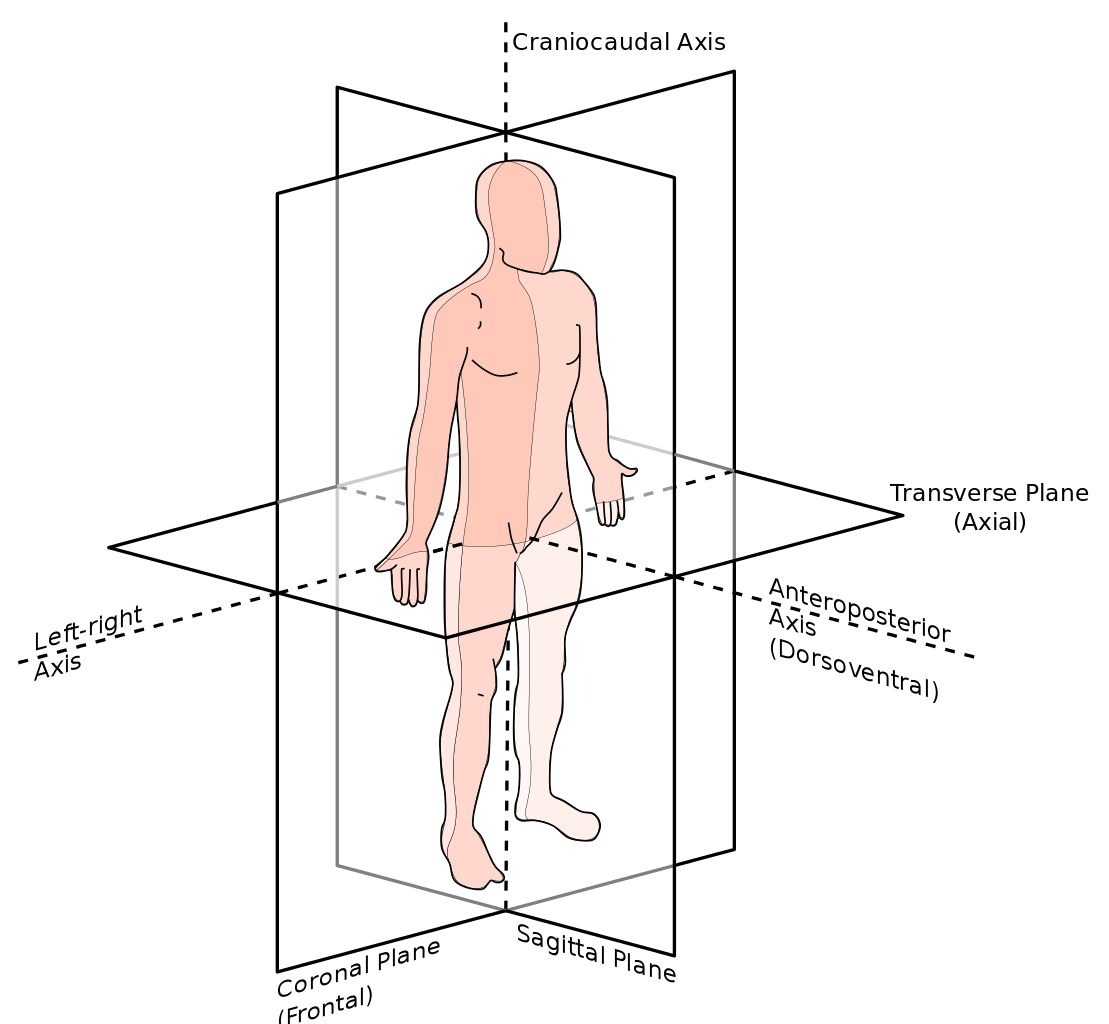
\includegraphics[width=10cm]{/home/thesis/images/Anatomical_Planes.png}
  \caption{Clarification of the terms regarding the anatomical planes
  }
\end{SCfigure}

\begin{SCfigure}[][htb]
  \centering
  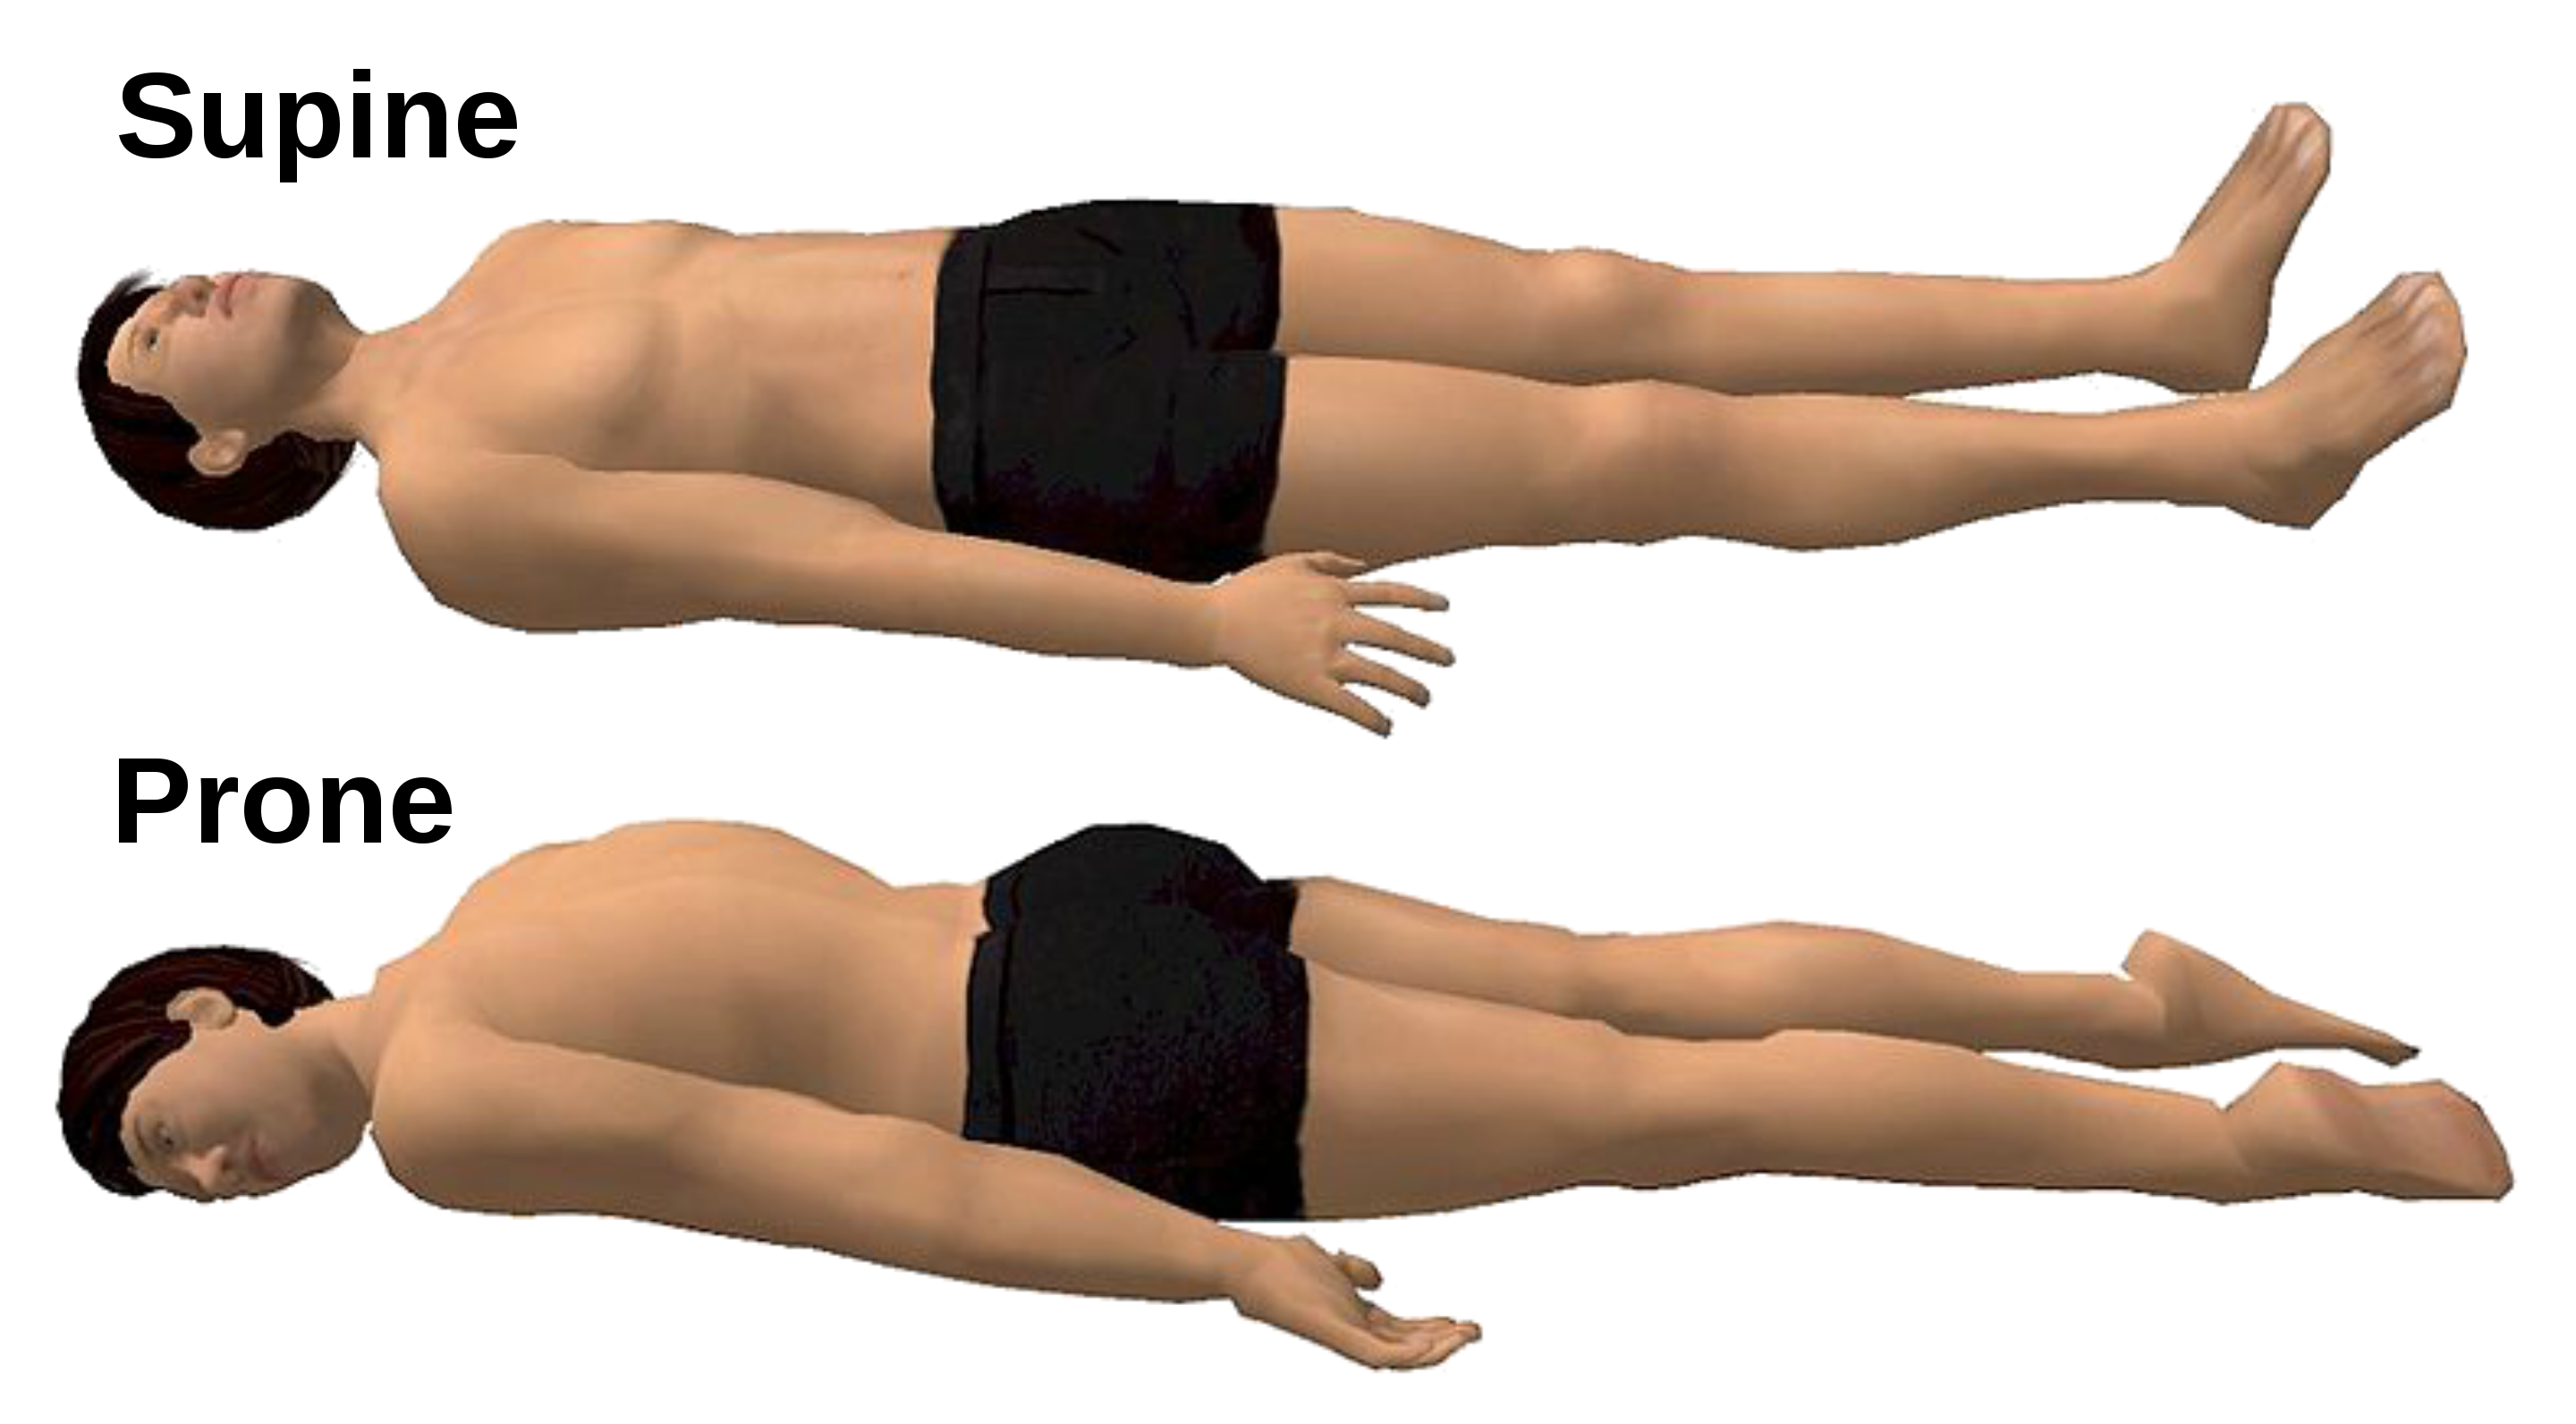
\includegraphics[width=10cm]{/home/thesis/images/prone_supine.png}
  \caption{Supine (face-up) and Prone (face-down) position of a patient.}
\end{SCfigure}

\chapter{Used software}

\todo[inline]{Software environments can be build with dockerfiles available in folder \textit{/dockerfiles/code/} of the git.}

\todo[inline]{Assure proper referencing of all libraries used}

\begin{SCtable}[\sidecaptionrelwidth][h]
 
  \begin{tabular}{ p{6cm} l l } 
   \hline
   \hline
   Library & version & reference  \\
   \hline 
   PyTorch & 1.7.1 &  \\ 
   SimpleITK &  &  \\ 
   \hline
   \hline
  \end{tabular}
  \caption{Python libraries used}

\end{SCtable}
\newgeometry{total={210mm,297mm},left=30mm,right=30mm,bindingoffset=5mm, top=25mm,bottom=25mm}
\chapter{Dataset agreements\label{seg:datasetagreement}}


\includegraphics[width=17cm]{/home/thesis/images/AgreementxVertSeg.png}